\documentclass{standalone}
\usepackage{tikz}
\usepackage{xcolor}
\usetikzlibrary{patterns, positioning}
\usetikzlibrary{shapes.misc}
\usepackage[outline]{contour}
\contourlength{1.5pt} 


\begin{document}
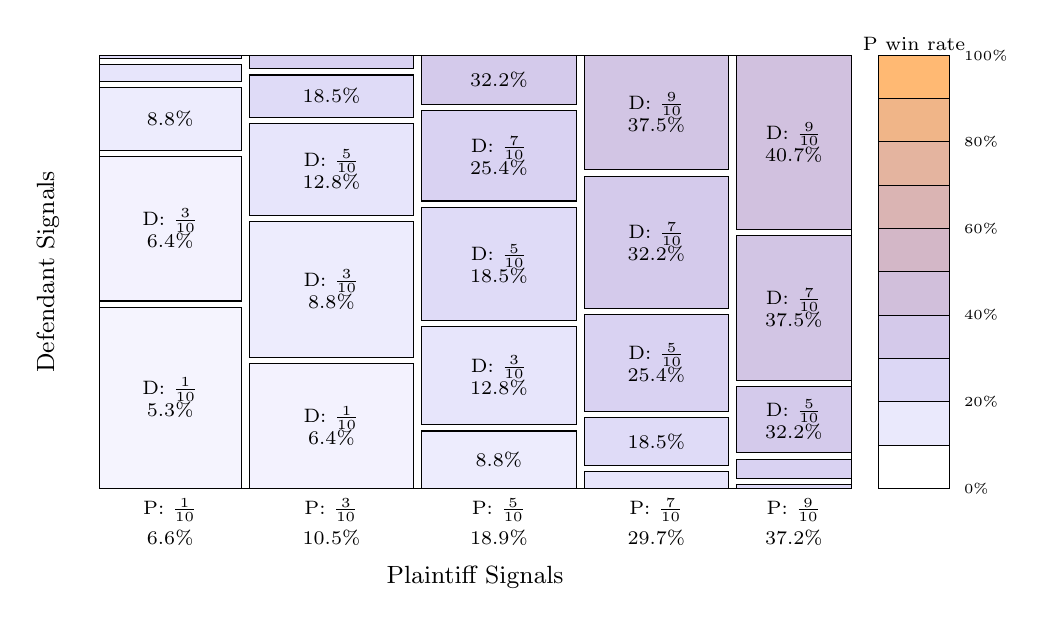
\begin{tikzpicture}
\newcommand{\DFractionOffset}{0.4}
\newcommand{\AxisLabelYAdjust}{-0.235}
\draw[draw=black] (0.6,2) rectangle (10.15,7.5);
\draw[fill=blue!95!orange!5!white!86!white, draw=black] (0.6,2) rectangle (2.4048,4.2999);
\draw (1.502419991412879, 3.1499323618668194) node[font=\scriptsize, text=black, align=center] {D: $\frac{1}{10}$\\ 5.3\%};
\draw[fill=blue!94!orange!6!white!86!white, draw=black] (0.6,4.3799) rectangle (2.4048,6.2142);
\draw (1.502419991412879, 5.2970238038638815) node[font=\scriptsize, text=black, align=center] {D: $\frac{3}{10}$\\ 6.4\%};
\draw[fill=blue!91!orange!9!white!85!white, draw=black] (0.6,6.2942) rectangle (2.4048,7.0877);
\draw (1.502419991412879, 6.690937294789257) node[font=\scriptsize, text=black, align=center] {8.8\%};
\draw[fill=blue!87!orange!13!white!84!white, draw=black] (0.6,7.1677) rectangle (2.4048,7.3812);
\draw[fill=blue!81!orange!19!white!82!white, draw=black] (0.6,7.4612) rectangle (2.4048,7.5);
\draw (1.502419991412879, 1.6) node[anchor=north, font=\scriptsize, text=black] {6.6\%};
\draw (1.502419991412879, {1.6 + \DFractionOffset}) node[anchor=north, font=\scriptsize, text=black] {P: $\frac{1}{10}$};
\draw[fill=blue!94!orange!6!white!86!white, draw=black] (2.5048,2) rectangle (4.5954,3.5836);
\draw (3.550129126159122, 2.791802626568962) node[font=\scriptsize, text=black, align=center] {D: $\frac{1}{10}$\\ 6.4\%};
\draw[fill=blue!91!orange!9!white!85!white, draw=black] (2.5048,3.6636) rectangle (4.5954,5.3861);
\draw (3.550129126159122, 4.52483910778783) node[font=\scriptsize, text=black, align=center] {D: $\frac{3}{10}$\\ 8.8\%};
\draw[fill=blue!87!orange!13!white!84!white, draw=black] (2.5048,5.4661) rectangle (4.5954,6.6338);
\draw (3.550129126159122, 6.049933936323666) node[font=\scriptsize, text=black, align=center] {D: $\frac{5}{10}$\\ 12.8\%};
\draw[fill=blue!81!orange!19!white!82!white, draw=black] (2.5048,6.7138) rectangle (4.5954,7.25);
\draw (3.550129126159122, 6.9818995447135075) node[font=\scriptsize, text=black, align=center] {18.5\%};
\draw[fill=blue!75!orange!25!white!80!white, draw=black] (2.5048,7.33) rectangle (4.5954,7.5);
\draw (3.550129126159122, 1.6) node[anchor=north, font=\scriptsize, text=black] {10.5\%};
\draw (3.550129126159122, {1.6 + \DFractionOffset}) node[anchor=north, font=\scriptsize, text=black] {P: $\frac{3}{10}$};
\draw[fill=blue!91!orange!9!white!85!white, draw=black] (4.6954,2) rectangle (6.6585,2.7295);
\draw (5.676955138523544, 2.3647739817824776) node[font=\scriptsize, text=black, align=center] {8.8\%};
\draw[fill=blue!87!orange!13!white!84!white, draw=black] (4.6954,2.8095) rectangle (6.6585,4.0531);
\draw (5.676955138523544, 3.43133157299929) node[font=\scriptsize, text=black, align=center] {D: $\frac{3}{10}$\\ 12.8\%};
\draw[fill=blue!81!orange!19!white!82!white, draw=black] (4.6954,4.1331) rectangle (6.6585,5.5693);
\draw (5.676955138523544, 4.8511887344915054) node[font=\scriptsize, text=black, align=center] {D: $\frac{5}{10}$\\ 18.5\%};
\draw[fill=blue!75!orange!25!white!80!white, draw=black] (4.6954,5.6493) rectangle (6.6585,6.7961);
\draw (5.676955138523544, 6.222674345911491) node[font=\scriptsize, text=black, align=center] {D: $\frac{7}{10}$\\ 25.4\%};
\draw[fill=blue!68!orange!32!white!77!white, draw=black] (4.6954,6.8761) rectangle (6.6585,7.5);
\draw (5.676955138523544, 7.188043202636798) node[font=\scriptsize, text=black, align=center] {32.2\%};
\draw (5.676955138523544, 1.6) node[anchor=north, font=\scriptsize, text=black] {18.9\%};
\draw (5.676955138523544, {1.6 + \DFractionOffset}) node[anchor=north, font=\scriptsize, text=black] {P: $\frac{5}{10}$};
\draw[fill=blue!87!orange!13!white!84!white, draw=black] (6.7585,2) rectangle (8.5938,2.21);
\draw[fill=blue!81!orange!19!white!82!white, draw=black] (6.7585,2.29) rectangle (8.5938,2.9008);
\draw (7.67612405056343, 2.595366504824214) node[font=\scriptsize, text=black, align=center] {18.5\%};
\draw[fill=blue!75!orange!25!white!80!white, draw=black] (6.7585,2.9808) rectangle (8.5938,4.2075);
\draw (7.67612405056343, 3.5941137821870206) node[font=\scriptsize, text=black, align=center] {D: $\frac{5}{10}$\\ 25.4\%};
\draw[fill=blue!68!orange!32!white!77!white, draw=black] (6.7585,4.2875) rectangle (8.5938,5.9654);
\draw (7.67612405056343, 5.126444497821166) node[font=\scriptsize, text=black, align=center] {D: $\frac{7}{10}$\\ 32.2\%};
\draw[fill=blue!63!orange!37!white!76!white, draw=black] (6.7585,6.0454) rectangle (8.5938,7.5);
\draw (7.67612405056343, 6.77271507839839) node[font=\scriptsize, text=black, align=center] {D: $\frac{9}{10}$\\ 37.5\%};
\draw (7.67612405056343, 1.6) node[anchor=north, font=\scriptsize, text=black] {29.7\%};
\draw (7.67612405056343, {1.6 + \DFractionOffset}) node[anchor=north, font=\scriptsize, text=black] {P: $\frac{7}{10}$};
\draw[fill=blue!81!orange!19!white!82!white, draw=black] (8.6938,2) rectangle (10.15,2.0481);
\draw[fill=blue!75!orange!25!white!80!white, draw=black] (8.6938,2.1281) rectangle (10.15,2.3721);
\draw[fill=blue!68!orange!32!white!77!white, draw=black] (8.6938,2.4521) rectangle (10.15,3.2932);
\draw (9.421878046786127, 2.872669046203804) node[font=\scriptsize, text=black, align=center] {D: $\frac{5}{10}$\\ 32.2\%};
\draw[fill=blue!63!orange!37!white!76!white, draw=black] (8.6938,3.3732) rectangle (10.15,5.2064);
\draw (9.421878046786127, 4.289776164480274) node[font=\scriptsize, text=black, align=center] {D: $\frac{7}{10}$\\ 37.5\%};
\draw[fill=blue!59!orange!41!white!75!white, draw=black] (8.6938,5.2864) rectangle (10.15,7.5);
\draw (9.421878046786127, 6.393176659801243) node[font=\scriptsize, text=black, align=center] {D: $\frac{9}{10}$\\ 40.7\%};
\draw (9.421878046786127, 1.6) node[anchor=north, font=\scriptsize, text=black] {37.2\%};
\draw (9.421878046786127, {1.6 + \DFractionOffset}) node[anchor=north, font=\scriptsize, text=black] {P: $\frac{9}{10}$};
\node[font=\small, text=black] at (5.375, {1.1 + \AxisLabelYAdjust}) {Plaintiff Signals};
\node[font=\small, text=black, rotate=90] at (-0.050000000000000044, 4.75) {Defendant Signals};
\draw[draw=black] (10.5,2) rectangle (11.4,7.5);
\draw (10.95, 7.65) node[font=\scriptsize, text=black] {P win rate};
\draw[fill=blue!100!orange!0!white!88!white, draw=black] (10.5,2) rectangle (11.4,2.55);
\draw[fill=blue!89!orange!11!white!84!white, draw=black] (10.5,2.55) rectangle (11.4,3.1);
\draw[fill=blue!78!orange!22!white!81!white, draw=black] (10.5,3.1) rectangle (11.4,3.65);
\draw[fill=blue!67!orange!33!white!77!white, draw=black] (10.5,3.65) rectangle (11.4,4.2);
\draw[fill=blue!56!orange!44!white!73!white, draw=black] (10.5,4.2) rectangle (11.4,4.75);
\draw[fill=blue!44!orange!56!white!70!white, draw=black] (10.5,4.75) rectangle (11.4,5.3);
\draw[fill=blue!33!orange!67!white!66!white, draw=black] (10.5,5.3) rectangle (11.4,5.85);
\draw[fill=blue!22!orange!78!white!62!white, draw=black] (10.5,5.85) rectangle (11.4,6.4);
\draw[fill=blue!11!orange!89!white!59!white, draw=black] (10.5,6.4) rectangle (11.4,6.95);
\draw[fill=blue!0!orange!100!white!55!white, draw=black] (10.5,6.95) rectangle (11.4,7.5);
\draw (11.46, 2) node[anchor=west, font=\tiny, text=black] {0\%};
\draw (11.46, 3.1) node[anchor=west, font=\tiny, text=black] {20\%};
\draw (11.46, 4.2) node[anchor=west, font=\tiny, text=black] {40\%};
\draw (11.46, 5.3) node[anchor=west, font=\tiny, text=black] {60\%};
\draw (11.46, 6.4) node[anchor=west, font=\tiny, text=black] {80\%};
\draw (11.46, 7.5) node[anchor=west, font=\tiny, text=black] {100\%};


\end{tikzpicture}
\end{document}